\documentclass[main.tex]{subfiles}

\begin{document}

\section{Offer Network Specifciation}
An \textbf{offer network} instance can be formally modeled as a directed graph, $G$, where vertices $t \in T$ represent tasks, $u \in U$ users, and labeled directed edges $(t_a,t_b) : u_1$\footnote{Can be a hypergraph if one wants user nodes rather than labels.}\footnote{In the current implementation, actually a multigraph: there can be multiple edges ($t_a,t_b$).} represent an offer by user $u_1$ to do task $t_a$ in exchange requested task $t_b$. I will call edgesCall this the task-centric graph formulation.
\begin{center}
  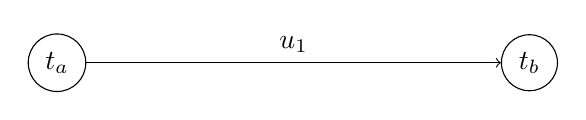
\begin{tikzpicture}
    \node[draw, circle] (ta) at (0,0) {$t_a$};
    \node[draw, circle] (tb) at (6,0) {$t_b$};
    \path [->] (ta) edge node[above] {$u_1$} (tb);
  \end{tikzpicture}
\end{center}

A matching of users who can satisfy each other is a vertex cycle. See the simplest case below:

\begin{center}
  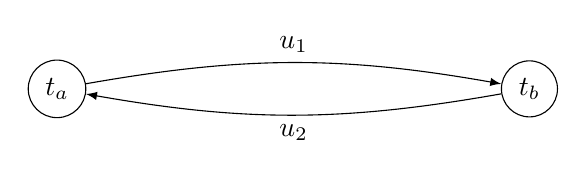
\begin{tikzpicture}
    \node[draw, circle] (ta) at (0,0) {$t_a$};
    \node[draw, circle] (tb) at (6,0) {$t_b$};
    \draw[-latex] (ta) to[bend left=10] node[above] {$u_1$} (tb);
    \draw[-latex] (tb) to[bend left=10] node[below] {$u_2$ }(ta);
  \end{tikzpicture}
\end{center}

\subsection{Dynamic Offer Network Specification}
The dynamic offer network is modeled in terms of discrete timesteps: $s = 0, 1, 2 \dots$.
Let $N_tt, N_d, N_m \in \mathbb{N}$, $p \in [0,1]$ be constants.

Between each timestep the following events can take place:
\begin{itemize}
  \item Add $N_tt$ new edges to the graph
  \item Remove $N_d$ unsatisfied edges
\end{itemize}

In addition every $N_m$ steps, an optimization algorithm is run in batch to suggest exchanges to users. An exchange is accepted if each edge is accepted by its user. Users accept the exchange for an edge with probability $p$. Rejected exchanges are left as is. All edges in accepted exchanges are removed from the graph.


\subsection{Additional Features}

The graph model can be made more sophisticated by drawing $N_tt$ and $N_d$ from a distribution, probabilistically adding new tasks, etc.

Below is a list of potentially desirable features of an offer network that don't qualify for an MVP:
\begin{itemize}
  \item Reputation biased matching
  \item Preferences for matching based on
    \begin{itemize}
      \item User preferences
      \item Task prefreences
    \end{itemize}
  \item ORs and ANDs of offers or request
\end{itemize}


\end{document}
